\subsection{Salient Social Activities Discovery and Prediction}
\label{sec:activity}

The joint target recognition problem described in the previous section represent one scenario where social contexts significantly assist and improve a traditional computer vision task. In this section, we propose a \emph{new} computer vision task motivated and enabled by socialized metadata. This new task introduces new `words' that a picture or a video may convey, and the output conversely produces new clues for social sensing in related disciplines. 

As the second major problem regarding socially-aware visual understanding, we propose to discover and predict salient social activities from videos, as well as still images if possible. The proposed task is novel from existing activity analysis and recognition work in three aspects: It seeks to discover salient social behaviors,  it  aims to predict activities using social contexts, and it directly builds upon realistic visual materials `in the wild'.

\begin{figure}[t!]
\begin{center}
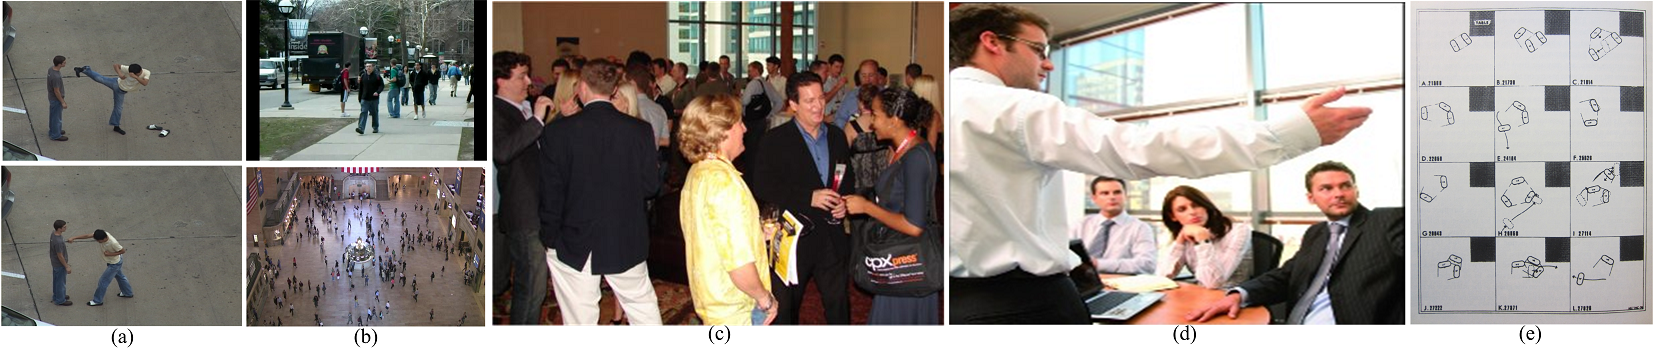
\includegraphics[width=\columnwidth]{socialbehavior}
\end{center}
\vspace{-0.25in} \caption{\captionsize 
(a): Socially non-informative co-occurrence of articulations\cite{UTdata}; (b): Socially non-informative collective crowd activities\cite{Choi:context,Choi:recogtrack}; (c): Socially informative salient interactions; (d) Socially informative salient group interactions in the nature; (e) Socially meaningful three-way activity categories defined as `f-formations' by sociology\cite{Kendon:book}.\label{fig:socialbehavior}\afterfigspace}
\end{figure}


First, we propose to discover salient social activities. Specifically, social semantics assist in visual understanding in the way that they provide new social behavior categories for us to distill from images and videos, and these new social categories are informed by qualitative and quantitative sociology, which has been studying these behavior modes but never be automated by computer vision. We refer to these new social semantics as salient. In contrast to existing vision research, salient social activities are distinctive because they do not focus on non-informative interactions or group-wise behaviors. The non-informative interactions, for example, refer to the co-occurrences of two individual body articulations with limited clue about how the two individuals are related or exchange opinions, such as 'kick', 'punch', etc. (\cite{UTdata}, Fig. \ref{fig:socialbehavior}(a)). The non-informative group-wise behaviors, on the other hand, include collective activities of a crowd, within which there are no explicit interactions, such as 'group-walking', 'queueing', etc. (\cite{Choi:context,Choi:recogtrack}, \ref{fig:socialbehavior}(b)). Instead, the salient social activities are more  of gestural and conversational interactions, attention-response, as well as turn-taking meetings  (Fig \ref{fig:socialbehavior}(c)) where sociological semantics, as is interesting and important to the sociology research, can be derived. Fig. \ref{fig:socialbehavior} (e) shows diagrams for such socially meaningful activities categories, namely `f-formations', in three-way interactions that have been under the investigation of sociology. Moreover, we will develop generic salient socialized discovering models and approaches, so that they accommodate activities of social populations of animals and insects (Fig. \ref{fig:socialbehavior}(d)).

Second, we propose to predict activities under social contexts. In this case, social semantics assist in visual understanding in the way that they serve as contextual information for restricting the more possible categories of activities that may occur between a specific group of individuals. This effort is also complementary to the usage of social contexts for identifying the targets presented in the previous section. Consider a simple illustrative example in which we would like to label a conversational scene in a movie as either a `negotiation� or a 'debate'. It is possible, in this case, that by the analysis of facial expressions, gestures, and poses, we still have difficulty in distinguishing the two. However, by appropriate face recognition in association with other metadata of the movie, probably with the help of social contexts as introduced in the previous section, we may gain solid confidence regarding the social relationship between the speakers as either `cooperative' or 'adverse'. A cooperative relationship are more likely to imply a negotiating activity, and an adverse relationship implies otherwise. A mechanism, similar to and in companion to the CRF formulation but adapted to video analysis, will be particularly useful.

Third, we expect to develop approaches that directly take in realistic visual materials recording social activities of interest. On the one hand, realistic visual materials capture the social activities in unconstrained environment in the format of long-term surveillance videos of public areas with irrelevant human beings co-existing with socially engaged actors as well as scene/background clutter. Our approach will be one that can effectively and efficiently localize and retrieve salient social activities in space and time from these large volumes of cluttered image sequences. On the other hand, realistic visual materials such as surveillance videos and web videos are frequently in low and varying frame-rate, in low resolution, blurry, as well as in adverse view-points. Our effort will be handling all these realistic conditions and providing robust and practical tools that process more than those simulated, high-quality, manually pre-processed data \cite{UTdata,Choi:context,Choi:recogtrack}.

\subsubsection{A prototype system and preliminary results}

\begin{figure}[t!]
\begin{center}
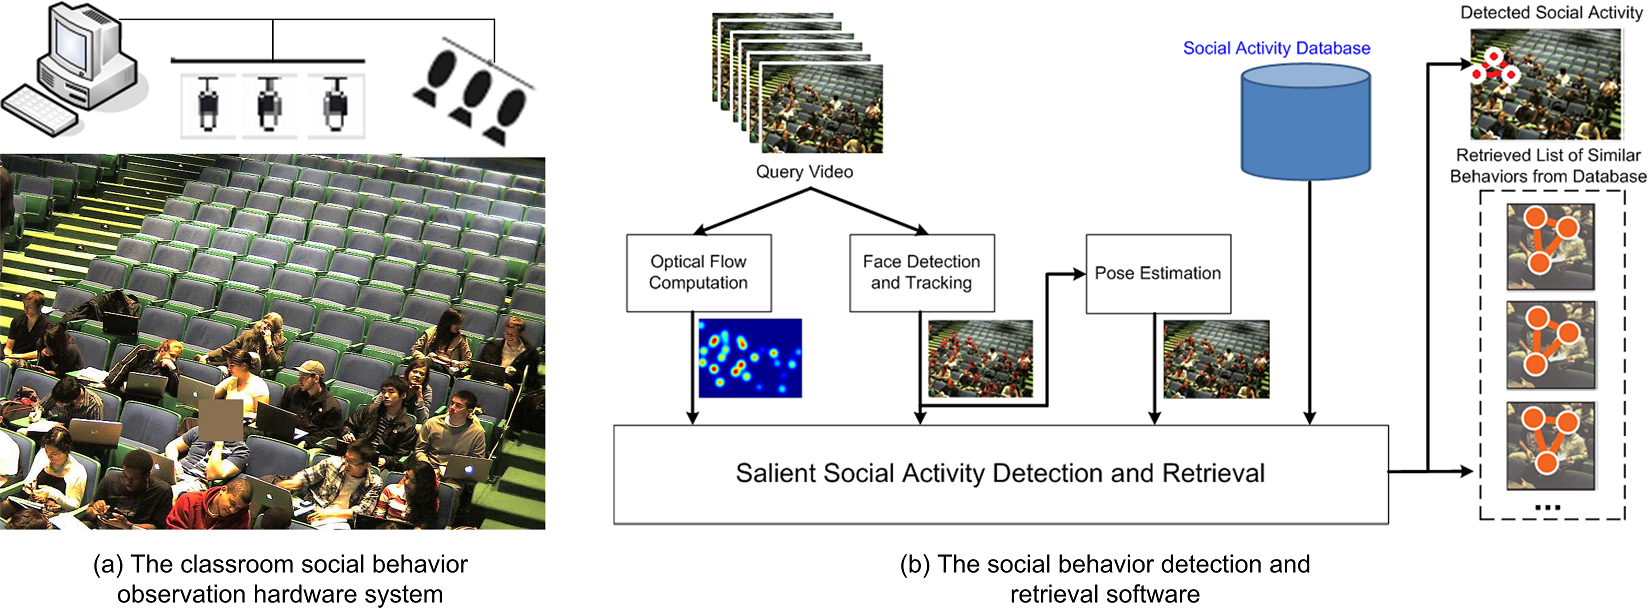
\includegraphics[width=\columnwidth]{prototype}
\end{center}
\vspace{-0.25in} \caption{\captionsize 
The prototype hardware and software infrastructure for analyzing socialized human behaviors in an indoor environment at Harvard University.\label{fig:prototype}\afterfigspace}
\end{figure}

As an initial attempt to analyze socialized human behaviors in an indoor environment, we have built up a prototype hardware and software infrastructure at Harvard University. As shown in Fig. \ref{fig:prototype}(a), the hardware part of the prototype system mainly consists of a networked audio-visual recording system for large-scale recording of student interactions in a Harvard College lecture hall. The system records audio and video from approximately one hundred students during each lecture in conjunction with the audience responses through an online teaching-learning application. The video system uses six IP cameras that together provide resolution that is high enough to achieve face-based identity recognition of each student in the audience. The audio system is an innovative design consisting 48 omnidirectional boundary microphones mounted inconspicuously among the seats, and outputting sound from each microphone recording to a single user-friendly mp3 audio file.To automatically analyze the videos, we have developed a robust computational suite of computer vision tools. This software consists of several fundamental modules that directly distill behavioral descriptions from raw videos, as well as a high-level module that detects salient social activities of interest from a new video and retrieves similar social activities. 


With this established classroom observation system and these fundamental modules, we have successfully collected and processed a large-scale classroom behavior database consisting of 100 video clips in total. The students are seated in a regular lecture hall and are observed by a camera array with non-overlapping fields of view. The classroom is ``interactive'' because at various times throughout the lecture students are invited to engage in ad-hoc group discussions about problems provided by the instructor. The scale of our database is orders of magnitude larger than state-of-the-art computer vision datasets (e.g. those used in \cite{UTdata,Choi:context,Choi:recogtrack}), in the number of individuals (10-50 students per camera), the number of cameras (6), and the amount of time (100 minutes per camera, per recording, equaling over 3,000 minutes in total). Through a combination of face detection and tracking, we obtained noisy tracks for all students in each monocular video, upon which we developed descriptive modules that directly extract descriptiors such as head pose and body motion, we have also implemented a high-level module for behavior analysis based on similarity between two social groups, as depicted in Fig. \ref{fig:prototype}(b). In this module, the behavior of each individual is represented by a combination of the head pose and the motion of torso and arms (using the method of histogram of optical flows). The social behavior of a group is then represented by the configuration in space and time of the behaviors of its participants. With this social activity representation, the module detects a salient social activity from a new video and retrieves similar social activities from our established database. This functionality is illustrated in Fig. \ref{fig:prototype}(b), where our system has discovered a three-way conversation by identifying the participants of this conversation and the time span (several to tens of seconds) of this event. Based on the behavior representation for this space-time social interaction, the system searches the remainder of the database and retrieves a list of exemplars containing similar social behavior, ranked in the descending order of the similarities with the query. In this way, any manual annotations associated with the query video can be propagated to the top-ranking exemplars, and we are now taking this approach to propagate our manual annotations across the whole database. 


\begin{figure}[t!]
\begin{center}
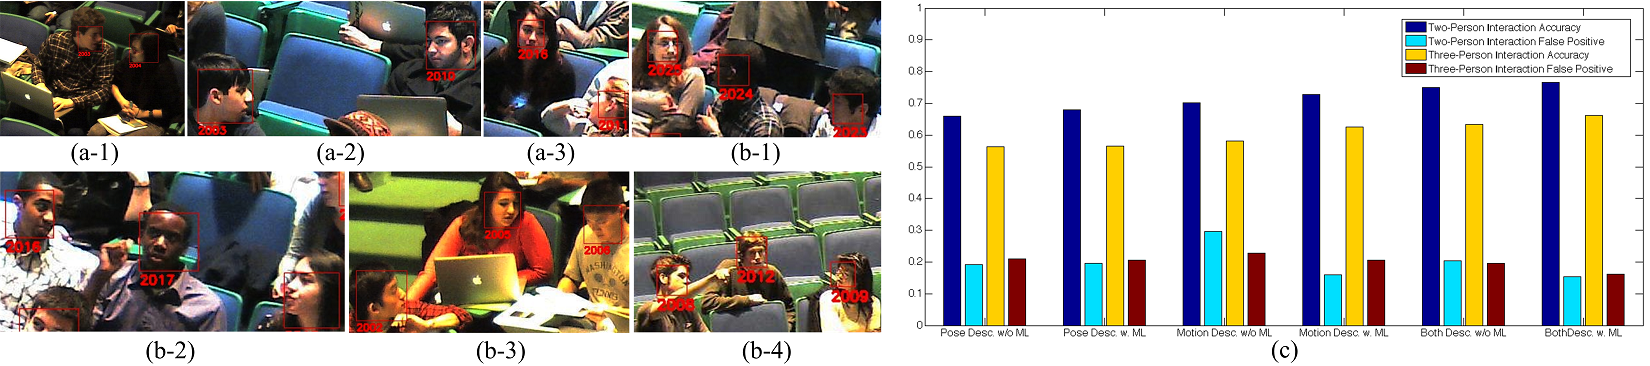
\includegraphics[width=\columnwidth]{dataset_compare}
\end{center}
\vspace{-0.25in} \caption{\captionsize 
(a-1)-(a-3): Examples of the three categories for two-person interactions; (b-1)-(b-4): Examples of the four categories for three-person interactions; (c) Preliminary performance comparisons of our social activity retrieval software.\label{fig:dataset_compare}\afterfigspace}
\end{figure}


To evaluate the effectiveness of the social behavior retrieval module, we manually identified the participants and start/end times of all two-person, three-person, and four-person interactions, obtaining 254 two-person and 112 three-person interactions in total to constitute the entire database. In consultation with education experts we define interaction categories based on the geometric configurations of the participants: three categories for 2-person interactions (same row; different rows with left agent in front; different rows with right agent in front) and four categories for 3-person interactions. Example images for each category can be found in Fig. \ref{fig:dataset_compare}(a)(b). The annotated interactions range from a few seconds to tens of seconds in length. Since the raw videos arise from five different hour-long session, and we adopt a leave-one-session-out evaluation scheme in partitioning training samples (exemplars) from test samples (inputs). We study classification performance for 2-person and 3-person interactions, where we measure the accuracy of inferred interaction categories. Our low-level modules include both pose descriptors and relative motion descriptors, and our high-level module employs Metric Learning (ML). To evaluate the effectiveness of all these functionalities, we turned off some of components as baselines and compared with the full module with all components on. Fig. \ref{fig:dataset_compare}(c) shows the average true positive rates vs. false positives when classifying detected interactions into the three or four categories. As expected we see that performance improves when more parts of the system turned on, which implies that our prototype infrastructure has achieved reasonable technical quality.

In our proposed research, we aim to enrich the descriptions of the social behaviors in the current prototype system, explore more accurate and robust comparison and retrieval mechanisms, and in particular, design novel modules for integrating social contextual annotations to allow our framework to be fully `socially-aware'.